\documentclass{standalone}

\usepackage{tikz}
\usetikzlibrary{decorations.pathreplacing,calligraphy}

\begin{document}
	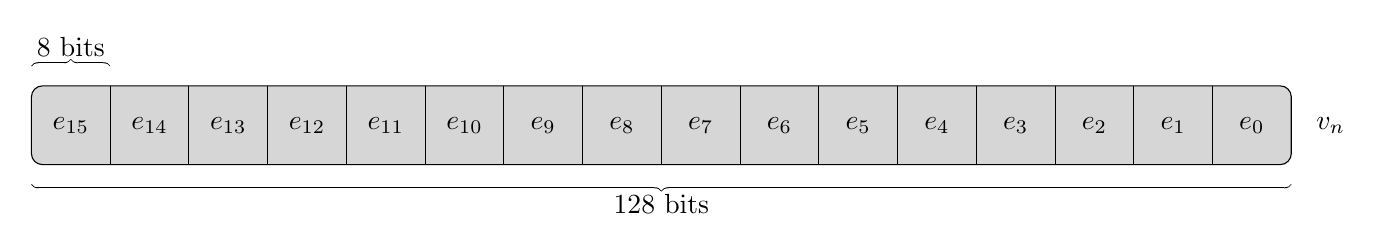
\begin{tikzpicture}
		%\draw[lightgray] (-2, -2) grid (18, 3);
		\draw[fill=gray!32, rounded corners] (0, 0) rectangle (16, 1);
		\draw (1, 0) -- (1, 1);
		\draw (2, 0) -- (2, 1);
		\draw (3, 0) -- (3, 1);
		\draw (4, 0) -- (4, 1);
		\draw (5, 0) -- (5, 1);
		\draw (6, 0) -- (6, 1);
		\draw (7, 0) -- (7, 1);
		\draw (8, 0) -- (8, 1);
		\draw (9, 0) -- (9, 1);
		\draw (10, 0) -- (10, 1);
		\draw (11, 0) -- (11, 1);
		\draw (12, 0) -- (12, 1);
		\draw (13, 0) -- (13, 1);
		\draw (14, 0) -- (14, 1);
		\draw (15, 0) -- (15, 1);
		
		\node at (0.5, 0.5) {$e_{15}$};
		\node at (1.5, 0.5) {$e_{14}$};
		\node at (2.5, 0.5) {$e_{13}$};
		\node at (3.5, 0.5) {$e_{12}$};
		\node at (4.5, 0.5) {$e_{11}$};
		\node at (5.5, 0.5) {$e_{10}$};
		\node at (6.5, 0.5) {$e_{9}$};
		\node at (7.5, 0.5) {$e_{8}$};
		\node at (8.5, 0.5) {$e_{7}$};
		\node at (9.5, 0.5) {$e_{6}$};
		\node at (10.5, 0.5) {$e_{5}$};
		\node at (11.5, 0.5) {$e_{4}$};
		\node at (12.5, 0.5) {$e_{3}$};
		\node at (13.5, 0.5) {$e_{2}$};
		\node at (14.5, 0.5) {$e_{1}$};
		\node at (15.5, 0.5) {$e_{0}$};
		
		\draw [decorate, decoration = {calligraphic brace}] (0, 1.25) --  (1, 1.25);
		\draw [decorate, decoration = {calligraphic brace, mirror}] (0, -0.25) --  (16, -0.25); 
		
		\node at (0.5, 1.5) {8 bits};
		\node at (8, -0.5) {128 bits};
		
		\node at (16.5, 0.5) {$v_{n}$};
	\end{tikzpicture}
\end{document}